\PassOptionsToPackage{dvipsnames}{xcolor}
%\documentclass[amsmath,table,sans,amsfonts, handout]{beamer}
\documentclass[amsmath,table,sans,amsfonts]{beamer}
\usepackage[T1]{fontenc}
%%\usepackage{beamerthemeshadow}
%%\usepackage[headheight=1pt,footheight=10pt]{beamerthemeboxes}
%%\addfootboxtemplate{\color{structure!80}}{\color{white}\tiny \hfill Karl Svozil (TU Vienna)\hfill}
%%\addfootboxtemplate{\color{structure!65}}{\color{white}\tiny \hfill mur.sat \hfill}
%%\addfootboxtemplate{\color{structure!50}}{\color{white}\tiny \hfill Graz, 2010-12-11\hfill}
%\usepackage[dark]{beamerthemesidebar}
%\usepackage[headheight=24pt,footheight=12pt]{beamerthemesplit}
%\usepackage{beamerthemesplit}
%\usepackage[bar]{beamerthemetree}
\usepackage{graphicx}

\usepackage{wrapfig,lipsum,booktabs}

%Global Background must be put in preamble
{%
%\usebackgroundtemplate%      \includegraphics[width=\paperwidth,height=\paperheight]{HaK-Urkaos-da}%
}
 \setbeamercolor{background canvas}{bg=black}

%\usepackage{eepic}
%\usepackage[usenames]{color}
%\newcommand{\Red}{\color{Red}}  %(VERY-Approx.PANTONE-RED)
%\newcommand{\Green}{\color{Green}}  %(VERY-Approx.PANTONE-GREEN)


%\RequirePackage[german]{babel}
%\selectlanguage{german}
%\RequirePackage[isolatin]{inputenc}

%\pgfdeclareimage[height=0.5cm]{logo}{tu-logo}
%\logo{\pgfuseimage{logo}}
\beamertemplatetriangleitem
%\beamertemplateballitem

\beamerboxesdeclarecolorscheme{alert}{red}{red!15!averagebackgroundcolor}
%\begin{beamerboxesrounded}[scheme=alert,shadow=true]{}
%\end{beamerboxesrounded}

%\beamersetaveragebackground{yellow!10}

%\beamertemplatecircleminiframe

\newtheorem{question}{Question}
\newtheorem{conjecture}[question]{Principle}
\newtheorem{challenge}[question]{Challenge}

\usepackage{tikz}
\usetikzlibrary{calc,decorations.pathreplacing,decorations.markings,positioning,shapes}




\definecolor{orange(webcolor)}{rgb}{1.0, 0.65, 0.0}
\setbeamercolor{normal text}{fg=white}
\setbeamercolor{structure}{fg=orange}

\setbeamertemplate{footline}
{
  \hbox{\begin{beamercolorbox}[wd=1\paperwidth,ht=2.25ex,dp=1ex,right]{framenumber}%
      \usebeamerfont{framenumber}\insertframenumber{} / \inserttotalframenumber\hspace*{2ex}
    \end{beamercolorbox}}%
  \vskip0pt%
}
\beamertemplatenavigationsymbolsempty

\setbeamersize{text margin left=0.5cm}

\begin{document}




\title{\bf \color{white} {Kolmogorov-type conditional probabilities among distinct context}   }
\subtitle{ \color{white}
\footnotesize http://tph.tuwien.ac.at/\textasciitilde{}svozil/publ/2019-Svozil-Prague-pres.pdf
 \\
\footnotesize based on https://arxiv.org/abs/1903.10424
}
\author{{Karl Svozil}}
\institute{{ITP/Vienna University of Technology, Austria\\
svozil@tuwien.ac.at
}
%{\tiny Disclaimer: Die hier vertretenen Meinungen des Autors verstehen sich als Diskussionsbeitr�ge und decken sich nicht notwendigerweise mit den Positionen der Technischen Universit�t Wien oder deren Vertreter.}
}
\date{\textcolor{white!100}{Prague, Czech Republic, May 18th, 2019}}

\maketitle

% \frame{
% \frametitle{}
%
% }

 \frame{
 \frametitle{Quantum bistochasticity}

In what follows any ``largest'' domain of mutually commuting observables will be termed {\em context}.
For quantum mechanics grounded in Hilbert space,
a context can be equivalently represented by
(i) an orthonormal basis,
(ii) the respective one-dimensional orthogonal projection operators associated with the basis elements,
or
(iii) a single maximal operator whose spectral sum is non-degenerated.

An essential assumption entering Gleason's derivation of the Born rule for quantum probabilities is the validity of classical probability theory
whenever the respective observables are co-measurable.
Formally, this amounts to the validity of Kolmogorov probability theory for mutually commuting observables;
and in particular, to the assumption of Kolmogorov's axioms within contexts.

}

 \frame{
 \frametitle{Quantum bistochasticity cntd.}

Consider two orthonormal bases aka two contexts.
Their respective conditional probabilities can be arranged into a matrix form:
The entry in the $i$-th row $j$-th column element corresponds to the conditional probability
associated with the probability of occurrence of the $j$-th element (observable) of the second context,
given the $i$-th element (observable)  of the first context.

By Gleason's assumption of the validity of Kolmogorov's axioms within contexts resulting in a conditional quantum probability
of the Born rule form,
as well as by
utilizing the dual role of projection operators in quantum mechanics as elementary two-valued observables as well as of pure states,
and by taking into account that cyclically interchanging factors inside a trace does not change its value,
this matrix needs to be doubly stochastic (bistochastic)
[Auffeves-Grangier-2017 DOI:10.1038/srep43365, Auffeves-Grangier-2018; DOI:10.1098/rsta.2017.0311];
that is, the sum taken within every single row and every single column adds up to one.

}

 \frame{
 \frametitle{Generalization of Kolmogorov axioms for multi-context environments}


In order to generalize the quantum case,
we suggest to postulate that the quantum case is just one instance satisfying a very general axiom:
That, given two arbitrary contexts
${\cal C}_1=\{ {\bf e}_1, \ldots {\bf e}_m\}$
and
${\cal C}_2=\{ {\bf f}_1, \ldots {\bf f}_n\}$,
the associated  $(n \times m)$-matrix whose entries are the conditional probabilities
$P( {\bf f}_j \vert {\bf e}_i )$
of ``${\bf f}_j$ given ${\bf e}_i$'' must be such that the sum taken within every single row adds up to one.
\begin{center}\color{orange}
$\widetilde{\qquad \qquad }$
$\widetilde{\qquad \qquad}$
$\widetilde{\qquad \qquad }$
\end{center}
{\footnotesize
We shall be mostly concerned with cases for which $n=m$;
that is, the associated matrix is a row (aka right) stochastic (square) matrix.
Formally,
such a matrix $\textsf{\textbf{A}}$ has nonnegative entries $a_{ij} \ge 0$ for $i,j =1,\ldots , n$ whose row sums
add up to one: $\sum_{j=1}^n a_{ij}=1$ for $i =1,\ldots , n$.
\begin{center}\color{orange}
$\widetilde{\qquad \qquad }$
$\widetilde{\qquad \qquad}$
$\widetilde{\qquad \qquad }$
\end{center}
The above criterium is a generalization of Kolmogorov's axioms, as it allows cases in which both contexts do not coincide.
For coinciding contexts this rule just reduces to Kolmogorov's axioms.
}
}


 \frame{
 \frametitle{Quasi-classical partition logics I: Two non-intertwining two-atomic contexts}
\begin{figure}[htpb]
\begin{center}
\begin{tabular}{cc}
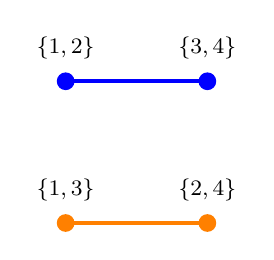
\begin{tikzpicture}  [scale=0.3]

\newdimen\ms
\ms=0.05cm

\tikzstyle{every path}=[line width=1.5pt]

\tikzstyle{c3}=[circle,inner sep={\ms/8},minimum size=4.5*\ms]
\tikzstyle{c2}=[circle,inner sep={\ms/8},minimum size=3*\ms]
\tikzstyle{c1}=[circle,inner sep={\ms/8},minimum size=1.5*\ms]


% Define positions of all observables
\path
  (0,0) coordinate(1)
  (6,0 ) coordinate(2)
  (0,6 ) coordinate(3)
  (6,6  ) coordinate(4)
;

% draw contexts

\draw [color=orange] (1) -- (2);
\draw [color=blue] (3) -- (4);


%
%%
%% draw atoms
%%
%
\draw (1) coordinate[c3,fill=orange,label={above:\footnotesize $\{1,3\}$}];   %
%
\draw (2) coordinate[c3,fill=orange,label={above:\footnotesize $\{2,4\}$}];    %
%
\draw (3) coordinate[c3,fill=blue,label={above:\footnotesize $\{1,2\}$}]; %
%
\draw (4) coordinate[c3,fill=blue,label={above:\footnotesize $\{3,4\}$}];  %
%
%

\end{tikzpicture}
&
\begin{tikzpicture}  [scale=0.3]

\newdimen\ms
\ms=0.05cm

\tikzstyle{every path}=[line width=1.5pt]

\tikzstyle{c3}=[circle,inner sep={\ms/8},minimum size=4.5*\ms]
\tikzstyle{c2}=[circle,inner sep={\ms/8},minimum size=3*\ms]
\tikzstyle{c1}=[circle,inner sep={\ms/8},minimum size=1.5*\ms]


% Define positions of all observables
\path
  (0,0) coordinate(1)
  (6,0 ) coordinate(2)
  (0,6 ) coordinate(3)
  (6,6  ) coordinate(4)
;

% draw contexts

\draw [color=orange] (1) -- (2);
\draw [color=blue] (3) -- (4);


%
%%
%% draw atoms
%%
%
\draw (1) coordinate[c3,fill=orange,label={above:\footnotesize $\frac{1}{\sqrt{2}}\begin{pmatrix}1,1\end{pmatrix}^\intercal$}];   %
%
\draw (2) coordinate[c3,fill=orange,label={above:\footnotesize $\frac{1}{\sqrt{2}}\begin{pmatrix}1,-1\end{pmatrix}^\intercal$}];    %
%
\draw (3) coordinate[c3,fill=blue,label={above:\footnotesize $\begin{pmatrix}1,0\end{pmatrix}^\intercal$}]; %
%
\draw (4) coordinate[c3,fill=blue,label={above:\footnotesize $\begin{pmatrix}0,1\end{pmatrix}^\intercal$}];  %
%
%

\end{tikzpicture}
\\
(a)&(b)
\end{tabular}
\end{center}
\caption{Greechie orthogonality diagram of a logic consisting of two nonintertwining contexts.
(a)
The associated (quasi)classical partition logic representations
obtained through in inverse construction using
all two-valued measures thereon (Svozil; DOI: 10.1007/s10773-005-7052-0);
(b) a faithful orthogonal representation (Lovasz, DOI: 10.1109/TIT.1979.1055985)
rendering a quantum {\it double}.
}
\label{2019-k-f1}
\end{figure}

}


 \frame{
 \frametitle{Quasi-classical partition logics I: Two non-intertwining two-atomic contexts cntd.}

{\footnotesize
This  logic  labels the atoms (aka elementary propositions)
obtained by an ``inverse construction''
using all two-valued measures thereon.
With the identifications
${\bf e}_1 \equiv \{1,2\}$,
${\bf e}_2 \equiv \{3,4\}$,
${\bf f}_1 \equiv \{1,3\}$, and
${\bf f}_2 \equiv \{2,4\}$
we obtain all classical probabilities
by identifying $i \rightarrow \lambda_i > 0$.
The respective conditional probabilities are
\begin{equation}
\begin{split}
\left[ P( {\cal C}_2 \vert {\cal C}_1 )\right] =
\left[ P( \{ {\bf f}_1, {\bf f}_2 \} \vert \{ {\bf e}_1,{\bf e}_2 ) \right]
\\
\equiv
\begin{pmatrix}
{P({\bf f}_1 \vert  {\bf e}_1)}  &  {P({\bf f}_2 \vert  {\bf e}_1)}      \\
{P({\bf f}_1 \vert  {\bf e}_2)}  &  {P({\bf f}_2 \vert  {\bf e}_2)}
\end{pmatrix}
=
\begin{pmatrix}
\frac{P({\bf f}_1 \cap {\bf e}_1)}{P({\bf e}_1)}  &  \frac{P({\bf f}_2 \cap {\bf e}_1)}{P({\bf e}_1)}      \\
\frac{P({\bf f}_1 \cap {\bf e}_2)}{P({\bf e}_2)}  &  \frac{P({\bf f}_2 \cap {\bf e}_2)}{P({\bf e}_2)}
\end{pmatrix}
\\
=
\begin{pmatrix}
\frac{P( \{1,3\}  \cap  \{1,2\} )}{P( \{1,2\} )}  &  \frac{P( \{2,4\}  \cap  \{1,2\} )}{P( \{1,2\} )}     \\
\frac{P( \{1,3\}  \cap  \{3,4\} )}{P( \{3,4\} )}  &  \frac{P( \{2,4\}  \cap  \{3,4\} )}{P( \{3,4\} )}
\end{pmatrix}
\\
=
\begin{pmatrix}
\frac{P( \{1\} )}{P( \{1,2\} )}  &  \frac{P( \{2\} )}{P( \{1,2\} )}   \\
\frac{P( \{3\} )}{P( \{3,4\} )}  &  \frac{P( \{4\} )}{P( \{3,4\} )}
\end{pmatrix}
=
\begin{pmatrix}
\frac{ \lambda_1 }{ \lambda_1+\lambda_2 }  &  \frac{ \lambda_2 }{ \lambda_1+\lambda_2 }     \\
\frac{ \lambda_3 }{ \lambda_3+\lambda_4 }  &  \frac{ \lambda_4 }{ \lambda_3+\lambda_4 }
\end{pmatrix},
\end{split}
\end{equation}
as well as
\begin{equation}
\begin{split}
\left[ P( {\cal C}_1 \vert {\cal C}_2 )\right] =
\left[ P( \{ {\bf e}_1, {\bf e}_2 \} \vert \{ {\bf f}_1,{\bf f}_2  \} ) \right]
\\
\equiv
%\begin{pmatrix}
%{P({\bf e}_1 \vert  {\bf f}_1)}  &  {P({\bf e}_2 \vert  {\bf f}_1)}        \\
%{P({\bf e}_1 \vert  {\bf f}_2)}  &  {P({\bf e}_2 \vert  {\bf f}_2)}
%\end{pmatrix}
%\\
%=
%\begin{pmatrix}
%\frac{P( \{1,2\}  \cap  \{1,3\} )}{P( \{1,3\} )}  &  \frac{P( \{3,4\}  \cap  \{1,3\} )}{P( \{1,3\} )}        \\
%\frac{P( \{1,2\}  \cap  \{2,4\} )}{P( \{2,4\} )}  &  \frac{P( \{3,4\}  \cap  \{2,4\} )}{P( \{2,4\} )}
%\end{pmatrix}
%\\
%=
\begin{pmatrix}
\frac{P( \{1\} )}{P( \{1,3\} )}  &  \frac{P( \{3\} )}{P( \{1,3\} )}      \\
\frac{P( \{2\} )}{P( \{2,4\} )}  &  \frac{P( \{4\} )}{P( \{2,4\} )}
\end{pmatrix}
=
\begin{pmatrix}
\frac{ \lambda_1 }{ \lambda_1+\lambda_3 }  &  \frac{ \lambda_3 }{ \lambda_1+\lambda_3 }       \\
\frac{ \lambda_2 }{ \lambda_2+\lambda_4 }  &  \frac{ \lambda_4 }{ \lambda_2+\lambda_4 }
\end{pmatrix}
.
\end{split}
\end{equation}
}
}

 \frame{
 \frametitle{Quasi-classical partition logics II: Two intertwining three-atomic contexts}

\begin{figure}[htpb]
\begin{center}
\begin{tabular}{cc}
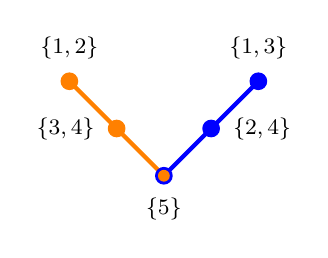
\begin{tikzpicture}  [scale=0.2]

\newdimen\ms
\ms=0.05cm

\tikzstyle{every path}=[line width=1.5pt]

\tikzstyle{c3}=[circle,inner sep={\ms/8},minimum size=4.5*\ms]
\tikzstyle{c2}=[circle,inner sep={\ms/8},minimum size=3*\ms]
\tikzstyle{c1}=[circle,inner sep={\ms/8},minimum size=1.5*\ms]

% Radius of regular polygons
\newdimen\R
\R=6cm     % outer circle

%\r= { \R * sqrt(3) }     % inner circle
%\newdimen\r
%\r=    {\R * sqrt(3)/2}       % inner circle

%\newdimen\K
%\K=3cm

% Define positions of all observables
\path
  (0,6 ) coordinate(1)
  (3,3    ) coordinate(2)
  (6,0 ) coordinate(3)
  (9,3) coordinate(4)
  (12,6  ) coordinate(5)
;

% draw contexts

\draw [color=orange] (1) -- (2) -- (3);
\draw [color=blue] (3) -- (4) -- (5);


%
%%
%% draw atoms
%%
%
\draw (1) coordinate[c3,fill=orange,label={above:\footnotesize $\{1,2\}$}];   %
%
\draw (2) coordinate[c3,fill=orange,label={left:\footnotesize $\{3,4\}$}];    %
%
\draw (3) coordinate[c3,fill=blue,label={below:\footnotesize $\{5\}$}]; %
\draw (3) coordinate[c2,fill=orange];  %
%
\draw (4) coordinate[c3,fill=blue,label={right:\footnotesize $\{2,4\}$}];  %
%
\draw (5) coordinate[c3,fill=blue,label={above:\footnotesize $\{1,3\}$}];  %
%
%

\end{tikzpicture}
&
\begin{tikzpicture}  [scale=0.2]

\newdimen\ms
\ms=0.05cm

\tikzstyle{every path}=[line width=1.5pt]

\tikzstyle{c3}=[circle,inner sep={\ms/8},minimum size=4.5*\ms]
\tikzstyle{c2}=[circle,inner sep={\ms/8},minimum size=3*\ms]
\tikzstyle{c1}=[circle,inner sep={\ms/8},minimum size=1.5*\ms]

% Radius of regular polygons
\newdimen\R
\R=6cm     % outer circle

%\r= { \R * sqrt(3) }     % inner circle
%\newdimen\r
%\r=    {\R * sqrt(3)/2}       % inner circle

%\newdimen\K
%\K=3cm

% Define positions of all observables
\path
  (0,6 ) coordinate(1)
  (3,3    ) coordinate(2)
  (6,0 ) coordinate(3)
  (9,3) coordinate(4)
  (12,6  ) coordinate(5)
;

% draw contexts

\draw [color=orange] (1) -- (2) -- (3);
\draw [color=blue] (3) -- (4) -- (5);


%
%%
%% draw atoms
%%
%
\draw (1) coordinate[c3,fill=orange,label={above:\footnotesize $\begin{pmatrix}1,0,0\end{pmatrix}^\intercal$}];   %
%
\draw (2) coordinate[c3,fill=orange,label={left:\footnotesize  $\begin{pmatrix}0,1,0\end{pmatrix}^\intercal$}];    %
%
\draw (3) coordinate[c3,fill=blue,label={below:\footnotesize    $\begin{pmatrix}0,0,1\end{pmatrix}^\intercal$}]; %
\draw (3) coordinate[c2,fill=orange];  %
%
\draw (4) coordinate[c3,fill=blue,label={right:\footnotesize    $\frac{1}{\sqrt{2}}\begin{pmatrix}1,1,0\end{pmatrix}^\intercal$}];  %
%
\draw (5) coordinate[c3,fill=blue,label={above:\footnotesize    $\frac{1}{\sqrt{2}}\begin{pmatrix}1,-1,0\end{pmatrix}^\intercal$}];  %
%
%

\end{tikzpicture}              6
\\
(a)&(b)
\end{tabular}
\end{center}
\caption{Greechie orthogonality diagram of  the $L_{12}$ ``firefly'' logic.
(a) The associated (quasi)classical partition logic representation
obtained through in inverse construction using all two-valued measures thereon (Svozil; DOI: 10.1007/s10773-005-7052-0);
(b) a faithful orthogonal representation (Lovasz, DOI: 10.1109/TIT.1979.1055985)
rendering a quantum {\it double}.
}
\label{2019-k-f-ffl}
\end{figure}

}

 \frame{
 \frametitle{Quasi-classical partition logics II: Two intertwining three-atomic contexts cntd.}

{
This  $L_{12}$ ``firefly'' logic  labels the atoms (aka elementary propositions)
obtained by an ``inverse construction''
using all two-valued measures thereon.
By design, it will be very similar to the earlier logic with four atoms.
With the identifications
${\bf e}_1 \equiv \{1,2\}$,
${\bf e}_2 \equiv \{3,4\}$,
${\bf e}_3 = {\bf f}_3 \equiv \{5\}$,
${\bf f}_1 \equiv \{1,3\}$, and
${\bf f}_2 \equiv \{2,4\}$
we obtain all classical probabilities
by identifying $i \rightarrow \lambda_i > 0$.
The respective conditional probabilities are
\begin{equation*}
\begin{split}
\left[ P( {\cal C}_2 \vert {\cal C}_1 )\right]
\equiv
%\begin{pmatrix}
%{P({\bf f}_1 \vert  {\bf e}_1)}  &  {P({\bf f}_2 \vert  {\bf e}_1)}   & {P({\bf f}_3 \vert  {\bf e}_1)}    \\
%{P({\bf f}_1 \vert  {\bf e}_2)}  &  {P({\bf f}_2 \vert  {\bf e}_2)}   & {P({\bf f}_3 \vert  {\bf e}_2)}    \\
%{P({\bf f}_1 \vert  {\bf e}_3)}  &  {P({\bf f}_2 \vert  {\bf e}_3)}   & {P({\bf f}_3 \vert  {\bf e}_3)}
%\end{pmatrix}
%\\
%=
%\begin{pmatrix}
%\frac{P({\bf f}_1 \cap {\bf e}_1)}{P({\bf e}_1)}  &  \frac{P({\bf f}_2 \cap {\bf e}_1)}{P({\bf e}_1)}   & \frac{P({\bf f}_3 \cap {\bf e}_1)}{P({\bf e}_1)}    \\
%\frac{P({\bf f}_1 \cap {\bf e}_2)}{P({\bf e}_2)}  &  \frac{P({\bf f}_2 \cap {\bf e}_2)}{P({\bf e}_2)}   & \frac{P({\bf f}_3 \cap {\bf e}_2)}{P({\bf e}_2)}    \\
%\frac{P({\bf f}_1 \cap {\bf e}_3)}{P({\bf e}_3)}  &  \frac{P({\bf f}_2 \cap {\bf e}_3)}{P({\bf e}_3)}   & \frac{P({\bf f}_3 \cap {\bf e}_3)}{P({\bf e}_3)}
%\end{pmatrix}
%\\
%=
%\begin{pmatrix}
%\frac{P( \{1,3\}  \cap  \{1,2\} )}{P( \{1,2\} )}  &  \frac{P( \{2,4\}  \cap  \{1,2\} )}{P( \{1,2\} )}   & \frac{P( \{5\}  \cap  \{1,2\} )}{P( \{1,2\} )}    \\
%\frac{P( \{1,3\}  \cap  \{3,4\} )}{P( \{3,4\} )}  &  \frac{P( \{2,4\}  \cap  \{3,4\} )}{P( \{3,4\} )}   & \frac{P( \{5\}  \cap  \{3,4\} )}{P( \{3,4\} )}    \\
%\frac{P( \{1,3\}  \cap  \{5\} )}{P( \{5\} )}  &  \frac{P( \{2,4\}  \cap  \{5\} )}{P( \{5\} )}   & \frac{P( \{5\}  \cap  \{5\} )}{P( \{5\} )}
%\end{pmatrix}
%\\
%=
\begin{pmatrix}
\frac{P( \{1\} )}{P( \{1,2\} )}  &  \frac{P( \{2\} )}{P( \{1,2\} )}   & \frac{P( \emptyset )}{P( \{1,2\} )}    \\
\frac{P( \{3\} )}{P( \{3,4\} )}  &  \frac{P( \{4\} )}{P( \{3,4\} )}   & \frac{P( \emptyset  )}{P( \{3,4\} )}    \\
\frac{P( \emptyset  )}{P( \{5\} )}  &  \frac{P( \emptyset  )}{P( \{5\} )}   & \frac{P( \{5\} )}{P( \{5\} )}
\end{pmatrix}
=
\begin{pmatrix}
\frac{ \lambda_1 }{ \lambda_1+\lambda_2 }  &  \frac{ \lambda_2 }{ \lambda_1+\lambda_2 }   & 0    \\
\frac{ \lambda_3 }{ \lambda_3+\lambda_4 }  &  \frac{ \lambda_4 }{ \lambda_3+\lambda_4 }   & 0    \\
0  &  0   & 1
\end{pmatrix},
\\
\left[ P( {\cal C}_1 \vert {\cal C}_2 )\right]
\equiv
%\begin{pmatrix}
%{P({\bf e}_1 \vert  {\bf f}_1)}  &  {P({\bf e}_2 \vert  {\bf f}_1)}   & {P({\bf e}_3 \vert  {\bf f}_1)}    \\
%{P({\bf e}_1 \vert  {\bf f}_2)}  &  {P({\bf e}_2 \vert  {\bf f}_2)}   & {P({\bf e}_3 \vert  {\bf f}_2)}    \\
%{P({\bf e}_1 \vert  {\bf f}_3)}  &  {P({\bf e}_2 \vert  {\bf f}_3)}   & {P({\bf e}_3 \vert  {\bf f}_3)}
%\end{pmatrix}
%\\
%=
%\begin{pmatrix}
%\frac{P({\bf e}_1 \cap {\bf f}_1)}{P({\bf f}_1)}  &  \frac{P({\bf e}_2 \cap {\bf f}_1)}{P({\bf f}_1)}   & \frac{P({\bf e}_3 \cap {\bf f}_1)}{P({\bf f}_1)}    \\
%\frac{P({\bf e}_1 \cap {\bf f}_2)}{P({\bf f}_2)}  &  \frac{P({\bf e}_2 \cap {\bf f}_2)}{P({\bf f}_2)}   & \frac{P({\bf e}_3 \cap {\bf f}_2)}{P({\bf f}_2)}    \\
%\frac{P({\bf e}_1 \cap {\bf f}_3)}{P({\bf f}_3)}  &  \frac{P({\bf e}_2 \cap {\bf f}_3)}{P({\bf f}_3)}   & \frac{P({\bf e}_3 \cap {\bf f}_3)}{P({\bf f}_3)}
%\end{pmatrix}
%\\
%=
%\begin{pmatrix}
%\frac{P( \{1,2\}  \cap  \{1,3\} )}{P( \{1,3\} )}  &  \frac{P( \{3,4\}  \cap  \{1,3\} )}{P( \{1,3\} )}   & \frac{P( \{5\}  \cap  \{1,3\} )}{P( \{1,3\} )}    \\
%\frac{P( \{1,2\}  \cap  \{2,4\} )}{P( \{2,4\} )}  &  \frac{P( \{3,4\}  \cap  \{2,4\} )}{P( \{2,4\} )}   & \frac{P( \{5\}  \cap  \{2,4\} )}{P( \{2,4\} )}    \\
%\frac{P( \{1,2\}  \cap  \{5\} )}{P( \{5\} )}  &  \frac{P( \{3,4\}  \cap  \{5\} )}{P( \{5\} )}   & \frac{P( \{5\}  \cap  \{5\} )}{P( \{5\} )}
%\end{pmatrix}
%\\
%=
\begin{pmatrix}
\frac{P( \{1\} )}{P( \{1,3\} )}  &  \frac{P( \{3\} )}{P( \{1,3\} )}   & \frac{P( \emptyset )}{P( \{1,3\} )}    \\
\frac{P( \{2\} )}{P( \{2,4\} )}  &  \frac{P( \{4\} )}{P( \{2,4\} )}   & \frac{P( \emptyset  )}{P( \{2,4\} )}    \\
\frac{P( \emptyset  )}{P( \{5\} )}  &  \frac{P( \emptyset  )}{P( \{5\} )}   & \frac{P( \{5\} )}{P( \{5\} )}
\end{pmatrix}
=
\begin{pmatrix}
\frac{ \lambda_1 }{ \lambda_1+\lambda_3 }  &  \frac{ \lambda_3 }{ \lambda_1+\lambda_3 }   & 0    \\
\frac{ \lambda_2 }{ \lambda_2+\lambda_4 }  &  \frac{ \lambda_4 }{ \lambda_2+\lambda_4 }   & 0    \\
0  &  0   & 1
\end{pmatrix}
.
\end{split}
\end{equation*}

}

}


 \frame{
 \frametitle{Quasi-classical partition logics II:
Pentagon/pentagram/house logic with five cyclically intertwining three-atomic contexts}

By now it should be clear how classical conditional probabilities work on partition logics.
Consider the pentagon/pentagram/(orthomodular) house
logic in Fig.~\ref{2019-k-f-pentagon} labels the atoms (aka elementary propositions)
obtained by an ``inverse construction''
using all 11 two-valued measures thereon.
take, for example, one of the two contexts ${\cal C}_4=\{  \{ 2,7,8\}, \{ 1,3,9,10,11 \}, \{  4,5,6 \} \}$ ``opposite'' to the context
${\cal C}_1=\{  \{ 1,2,3\}, \{ 4,5,7,9,11\}, \{  6,8,10 \} \}$.



\begin{figure}[htpb]
\begin{center}
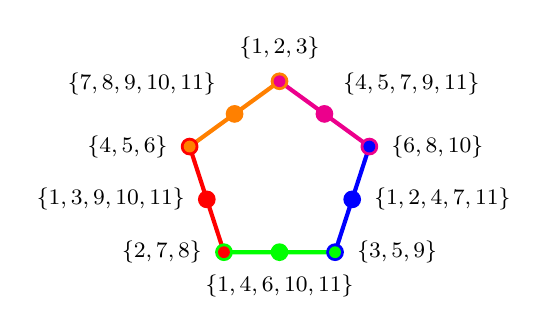
\begin{tikzpicture}  [scale=0.2]

\newdimen\ms
\ms=0.05cm

\tikzstyle{every path}=[line width=1.5pt]

\tikzstyle{c3}=[circle,inner sep={\ms/8},minimum size=4.5*\ms]
\tikzstyle{c2}=[circle,inner sep={\ms/8},minimum size=3*\ms]
\tikzstyle{c1}=[circle,inner sep={\ms/8},minimum size=1.5*\ms]

% Radius of regular polygons
\newdimen\R
\R=6cm     % outer circle

%\r= { \R * sqrt(3) }     % inner circle
%\newdimen\r
%\r=    {\R * sqrt(3)/2}       % inner circle

%\newdimen\K
%\K=3cm

% Define positions of all observables
\path
  ({90 + 0 * 360 /5}:\R      ) coordinate(1)
  ({90 + 36 + 0 * 360 /5}:{\R * sqrt((25+10*sqrt(5))/(50+10*sqrt(5)))}      ) coordinate(2)
  ({90 + 1 * 360 /5}:\R   ) coordinate(3)
  ({90 + 36 + 1 * 360 /5}:{\R * sqrt((25+10*sqrt(5))/(50+10*sqrt(5)))}   ) coordinate(4)
  ({90 + 2 * 360 /5}:\R  ) coordinate(5)
  ({90 + 36 + 2 * 360 /5}:{\R * sqrt((25+10*sqrt(5))/(50+10*sqrt(5)))}  ) coordinate(6)
  ({90 + 3 * 360 /5}:\R  ) coordinate(7)
  ({90 + 36 + 3 * 360 /5}:{\R * sqrt((25+10*sqrt(5))/(50+10*sqrt(5)))}  ) coordinate(8)
  ({90 + 4 * 360 /5}:\R     ) coordinate(9)
  ({90 + 36 + 4 * 360 /5}:{\R * sqrt((25+10*sqrt(5))/(50+10*sqrt(5)))}     ) coordinate(10)
;

% draw contexts

\draw [color=orange] (1) -- (2) -- (3);
\draw [color=red] (3) -- (4) -- (5);
\draw [color=green] (5) -- (6) -- (7);
\draw [color=blue] (7) -- (8) -- (9);
\draw [color=magenta] (9) -- (10) -- (1);    %


%
%%
%% draw atoms
%%
%
\draw (1) coordinate[c3,fill=orange,label=90:{\footnotesize $\{ 1,2,3\} $}];   %
\draw (1) coordinate[c2,fill=magenta];  %
%
\draw (2) coordinate[c3,fill=orange,label={above left:\footnotesize $\{ 7,8,9,10,11\}$}];    %
%
\draw (3) coordinate[c3,fill=red,label={left:\footnotesize $\{ 4,5,6\} $}]; %
\draw (3) coordinate[c2,fill=orange];  %
%
\draw (4) coordinate[c3,fill=red,label={left:\footnotesize $\{ 1,3,9,10,11\}$}];  %
%
\draw (5) coordinate[c3,fill=green,label={left:\footnotesize $\{ 2,7,8\} $}];  %
\draw (5) coordinate[c2,fill=red];  %
%
\draw (6) coordinate[c3,fill=green,label={below:\footnotesize $\{ 1,4,6,10,11\} $}];
%
\draw (7) coordinate[c3,fill=blue,label={right:\footnotesize $\{ 3,5,9\}$}];  %
\draw (7) coordinate[c2,fill=green];  %
%
\draw (8) coordinate[c3,fill=blue,label={right:\footnotesize $\{ 1,2,4,7,11\}$}];  %
%
\draw (9) coordinate[c3,fill=magenta,label={right:\footnotesize $\{ 6,8,10\}$}];
\draw (9) coordinate[c2,fill=blue];  %
%
\draw (10) coordinate[c3,fill=magenta,label={above right:\footnotesize $\{ 4,5,7,9,11\}$}];  %
%
%
\end{tikzpicture}
\end{center}
\caption{Greechie orthogonality diagrams of   the pentagon/pentagram/house logic.
}
\label{2019-k-f-pentagon}
\end{figure}
}


 \frame{
 \frametitle{Quasi-classical partition logics II:
Pentagon/pentagram/house logic with five cyclically intertwining three-atomic contexts cntd.}
{\footnotesize

With the identifications
${\bf e}_1 \equiv \{1,2,3\}$,
${\bf e}_2 \equiv \{4,5,7,9,11\}$,
${\bf e}_3   \equiv \{6,8,10\}$,
${\bf f}_1 \equiv \{2,7,8\}$,
${\bf f}_2 \equiv \{1,3,9,10,11\}$, and
${\bf f}_3   \equiv \{4,5,6\}$.
The respective conditional probabilities are
\begin{equation*}
\begin{split}
\left[ P( {\cal C}_2 \vert {\cal C}_1 )\right] =
\left[ P( \{ {\bf f}_1, {\bf f}_2, {\bf f}_3 \} \vert \{ {\bf e}_1,{\bf e}_2,{\bf e}_3 \} ) \right]
\\
\equiv
%\begin{pmatrix}
%{P({\bf f}_1 \vert  {\bf e}_1)}  &  {P({\bf f}_2 \vert  {\bf e}_1)}   & {P({\bf f}_3 \vert  {\bf e}_1)}    \\
%{P({\bf f}_1 \vert  {\bf e}_2)}  &  {P({\bf f}_2 \vert  {\bf e}_2)}   & {P({\bf f}_3 \vert  {\bf e}_2)}    \\
%{P({\bf f}_1 \vert  {\bf e}_3)}  &  {P({\bf f}_2 \vert  {\bf e}_3)}   & {P({\bf f}_3 \vert  {\bf e}_3)}
%\end{pmatrix}
%=
%\begin{pmatrix}
%\frac{P({\bf f}_1 \cap {\bf e}_1)}{P({\bf e}_1)}  &  \frac{P({\bf f}_2 \cap {\bf e}_1)}{P({\bf e}_1)}   & \frac{P({\bf f}_3 \cap {\bf e}_1)}{P({\bf e}_1)}    \\
%\frac{P({\bf f}_1 \cap {\bf e}_2)}{P({\bf e}_2)}  &  \frac{P({\bf f}_2 \cap {\bf e}_2)}{P({\bf e}_2)}   & \frac{P({\bf f}_3 \cap {\bf e}_2)}{P({\bf e}_2)}    \\
%\frac{P({\bf f}_1 \cap {\bf e}_3)}{P({\bf e}_3)}  &  \frac{P({\bf f}_2 \cap {\bf e}_3)}{P({\bf e}_3)}   & \frac{P({\bf f}_3 \cap {\bf e}_3)}{P({\bf e}_3)}
%\end{pmatrix}
%\\
%=
\begin{pmatrix}
\frac{P( \{2,7,8\}  \cap  \{1,2,3\} )}{P( \{1,2,3\} )} &  \frac{P( \{1,3,9,10,11\}  \cap  \{1,2,3\} )}{P( \{1,2,3\} )} &  \frac{P( \{4,5,6\}  \cap  \{1,2,3\} )}{P( \{1,2,3\} )}    \\
\frac{P( \{2,7,8\}  \cap  \{4,5,7,9,11\} )}{P( \{4,5,7,9,11\} )}  &  \frac{P( \{1,3,9,10,11\}  \cap  \{4,5,7,9,11\} )}{P( \{4,5,7,9,11\} )}   & \frac{P( \{4,5,6\}  \cap  \{4,5,7,9,11\} )}{P( \{4,5,7,9,11\} )}    \\
\frac{P( \{2,7,8\}  \cap  \{6,8,10\} )}{P( \{6,8,10\} )}  &  \frac{P( \{1,3,9,10,11\}  \cap  \{6,8,10\} )}{P( \{6,8,10\} )}   & \frac{P( \{4,5,6\}  \cap  \{6,8,10\} )}{P( \{6,8,10\} )}
\end{pmatrix}
\\
=
\begin{pmatrix}
\frac{P( \{2\} )}{P( \{1,2,3\} )}  &  \frac{P( \{1,3\} )}{P( \{1,2,3\} )}   & \frac{P( \emptyset)}{P( \{1,2,3\} )}    \\
\frac{P( \{7\} )}{P( \{4,5,7,9,11\} )}  &  \frac{P( \{11\} )}{P( \{4,5,7,9,11\} )}   & \frac{P( \{4,5 \} )}{P( \{4,5,7,9,11\} )}    \\
\frac{P( \{8\} )}{P( \{6,8,10\} )}  &  \frac{P( \{10\} )}{P( \{6,8,10\} )}   & \frac{P( \{6\} )}{P( \{6,8,10\} )}
\end{pmatrix}
\\
=
\begin{pmatrix}
\frac{ \lambda_2 }{ \lambda_1+\lambda_2 +\lambda_3}  &  \frac{ \lambda_1 + \lambda_3 }{\lambda_1+\lambda_2 +\lambda_3 }   &  0    \\
\frac{ \lambda_7 }{ \lambda_4+\lambda_5 + \lambda_7+\lambda_9 +\lambda_{11}  }  &  \frac{ \lambda_9 + \lambda_{11}}{ \lambda_4+\lambda_5 + \lambda_7+\lambda_9 +\lambda_{11}  }   & \frac{ \lambda_4+\lambda_5 }{ \lambda_4+\lambda_5 + \lambda_7+\lambda_9 +\lambda_{11}  }     \\
\frac{ \lambda_8 }{ \lambda_6+\lambda_8+\lambda_{10} }  &  \frac{ \lambda_{10} }{ \lambda_6+\lambda_8+\lambda_{10} }   & \frac{ \lambda_6 }{ \lambda_6+\lambda_8+\lambda_{10} }
\end{pmatrix}.
\end{split}
\end{equation*}
}
}

 \frame{
 \frametitle{Extrema of conditional probabilities in row and doubly stochastic matrices}

The row stochastic matrices representing conditional probabilities
form a polytope in $\mathbb{R}^{n^2}$ whose vertices
are the $n^n$ matrices $\textsf{\textbf{T}}_i$, $i= 1, \ldots , n^n$, with exactly one entry $1$ in each row.
Therefore, a row stochastic matrix can be represented as the convex sum $\sum_{i=1}^{n^n} \lambda_i \textsf{\textbf{T}}_i$,
with nonnegative $\lambda_i \ge 0$ and  $\sum_{i=1}^{n^n} \lambda_i =1$.

For conditional probabilities yielding doubly stochastic matrices, such as, for instance, the quantum case, the Birkhoff theorem
yields more restricted linear bounds:
it states that any doubly stochastic $(n\times n)$--matrix is the convex hull of $m\le (n-1)^2+1 \le n!$ permutation matrices.
That is, if $\textsf{\textbf{A}}\equiv a_{ij}$ is a doubly stochastic matrix such that $a_{ij} \ge 0$ and
$
\sum_{i=1}^n a_{ij}
=
\sum_{i=1}^n a_{ji}
=1
$ for $1\le i,j \le n$,
then there exists a convex sum decomposition
$\textsf{\textbf{A}} =\sum_{k=1}^{m \le (n-1)^2+1 \le n!}  \lambda_k \textsf{\textbf{P}}_k$
in terms of $m\le (n-1)^2+1$ linear independent permutation matrices
$\textsf{\textbf{P}}_k$
such that $\lambda_k \ge 0$ and $\sum_{k=1}^{m \le (n-1)^2+1 \le n!}  \lambda_k =1$.


}



\frame{

\centerline{\huge {\color{yellow} Thank you for your attention!}}

\begin{center}\color{orange}
$\widetilde{\qquad \qquad }$
$\widetilde{\qquad \qquad}$
$\widetilde{\qquad \qquad }$
\end{center}

 }
 \end{document}








 \frame{
 \frametitle{}

 }


